\section*{Appendix II - Gabor and Morlet Wavelets}
\subsection*{Gabor Wavelet filter}
The 1D-Gabor wavelet is defined spatially by
\begin{equation}
    \psi(x)=exp\left(-\frac{x^2}{2\sigma^2}+i\xi x\right)
    \label{eqn_app2_wfil00}
\end{equation}
The Fourier-transform is
\begin{equation}
    \hat{\psi}(\omega)=exp\left(-\frac{\sigma^2(\omega-\xi)^2}{2}\right)
    \label{eqn_app2_wfil01}
\end{equation}
It's value bounded at 0 is $\hat{\psi(0)}=exp(-\sigma^2\xi^2/2)$, so we have
\begin{equation}
    \xi\sigma=\sqrt{-2\log(\hat{\psi}(0))}
    \label{eqn_app2_wfil02}
\end{equation}
The wavelets are therefore computed as 
\begin{equation}
    \psi_j=\frac{1}{a^j\sigma}\left(\frac{x}{a^j}\right)
    \label{eqn_app2_wfil03}
\end{equation}

Where $a$ is the scale factor.  if we call $\tau$, the value of the two Gabor where the plots intersect, we have, as in figure \ref{fig_app2_gab}.
\begin{figure}
\centering
  % Requires \usepackage{graphicx}
  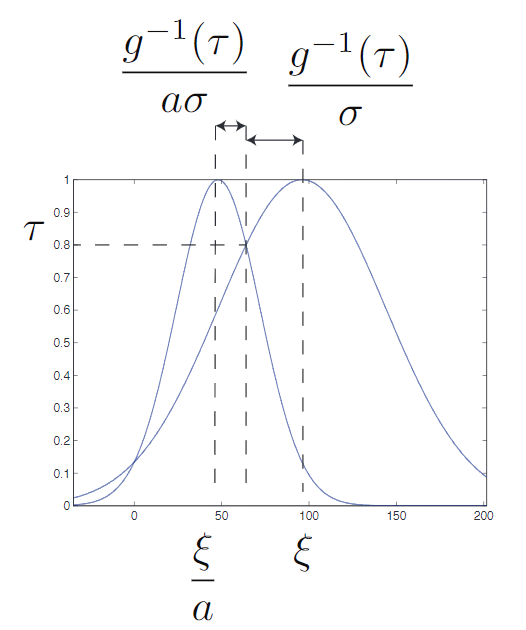
\includegraphics[width=14cm]{thesis/images/gab}\\
  \caption{Fourier transform of adjacent scale Gabor wavelet. $\tau$ has been set to 0.8} \label{fig_app2_gab}
\end{figure}
\begin{equation}
    \frac{\xi}{a}+\frac{g^{-1}(\tau)}{a\sigma}=\xi-\frac{g^{-1}(\tau)}{\sigma}
    \label{eqn_app2_wfil04}
\end{equation}
where $g(x)=exp(-x^2/2)$ i.e. $g^{-1}(\tau)=\sqrt{-2\log(\tau)}$
So we have
\begin{equation}
    \xi\sigma=\sqrt{-2\log(\tau)}\frac{a+1}{a-1}
    \label{eqn_app2_wfil05}
\end{equation}

The value of $\xi$ is fixed by the fact that we need the frequency information so we set 
\begin{equation}
    \xi=3\pi/4
    \label{eqn_app2_wfil06}
\end{equation}

Equations (\ref{eqn_app2_wfil02} and \ref{eqn_app2_wfil05}) show that the choice of $\sigma$ is  trade off between two antagonist requirement on the wavelet
\begin{enumerate}
    \item a zero-mean: $\sigma$ should be large.
    \item $tau$ should be large therefore $\sigma$ should be small
\end{enumerate}

With these requirements met we see that
\begin{equation}
    \hat{\psi}(0)=\tau^\frac{(a+1)^2}{(a-1)^2}
\end{equation}

So we can see that these two requirements are compatible as we take more and more bands per octave.

In the implementation, the only parameter about the wavelet that the user can set is $\tau_{as}=\tau$, where 'as' stands for adjacent scales.  The implementation of parameters is the following
\begin{enumerate}
    \item The value of $\xi$ is set to $3\pi/4$.
    \item The user chooses values for $\tau,a$ and $j$.
    \item The value of $\sigma$ is computed with
    \begin{equation}
        \sigma=\frac{\sqrt{-2\log(\tau)}}{\xi}\frac{a+1}{a-1}
    \end{equation}
\end{enumerate}

There is another parameter called $\tau_{lc}$.  'lc' stands for low-coarse.  It controls the value crossing between the low pass filters $\psi_j$ (a Gaussian) and the coarsest scale wavelet $\psi_{J-1}$ and this parameter determines the value of the bandwidth of the low pas filter.

\subsection*{Morlet wavelet filter}
Morlet filters are modified Gabor filters that have zero-mean:  The idea is to subtract a Gabor, its envelop times a constant so that the results has zero mean:
\begin{equation}
   \phi(x)=\exp\left(-\frac{x^2}{2\sigma^2}\right)(\exp(i\xi x)-exp(-\sigma^2\zi^2/2)) 
\end{equation}
It’s Fourier transform is
\begin{equation}
   \hat{\psi}(\omega)=\omega\left\exp\left(-\frac{\sigma^2(\omega-\xi)^2}{2}\right)-\exp\left(-\frac{\sigma^2(\omega+\xi)^2}{2}\right)\right) 
\end{equation}
And we can see it has zero $\hat{\psi}(0)=0$
\begin{figure}
\centering
  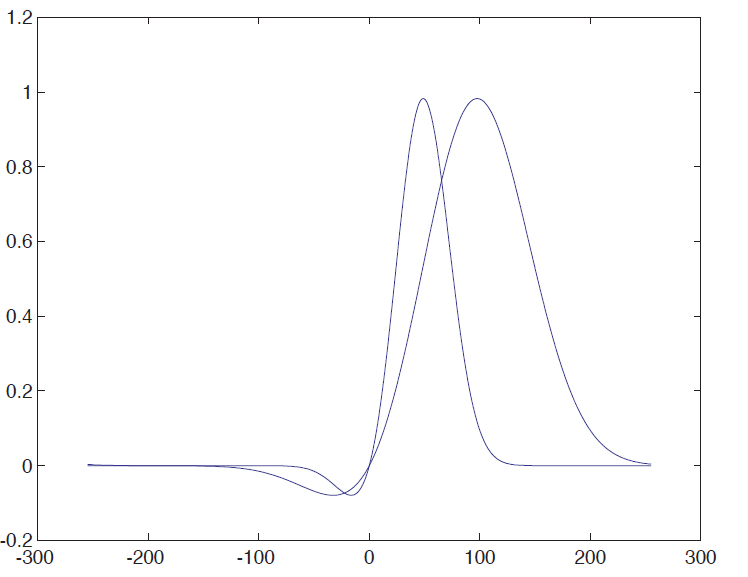
\includegraphics[width=14cm]{thesis/images/morlet}\\
  \caption{Fourier transform of adjacent scale Gabor wavelet. $\tau$ has been set to 0.8} \label{fig_app2_morlet}
\end{figure}
